\documentclass[10pt,a4paper]{article}
\usepackage[utf8]{inputenc}
\usepackage{amsmath}
\usepackage{amsfonts}
\usepackage{amssymb}
\usepackage{graphicx}
\usepackage[left=2cm,right=2cm,top=2cm,bottom=2cm]{geometry}
\author{Castro Mejia Jonatan Alejandro 314027687\\ Rosado cabrera Diego  314293804}

\title{Tarea 3 \\Criptografía y Seguridad \\ Curvas Elípticas}

\begin{document}
\maketitle
\begin{enumerate}
\item Sea E: $y^{2}+20x= x^{3}+21(mod 35)$ y sea Q =(15,-4) $\in$ E.
\begin{itemize}
\item[a)] Factoriza 35 tratando de calcular 3Q.
\\Hay que obtener 2Q, y esto es haciendo Q + Q, y como son iguales, entonces: $\lambda$ = (3x$_{1}^{2}$ + a)(2$y_{1})^{-1}$ 
\\Entonces $\lambda$ = (3(15)$^{2}$ - 20)(2(-4))$^{-1}$(-8$^{-1} \equiv $13 mod 35) = (675-20)(13) mod 35 = 655(13) = 8515 mod 35\\
$\lambda$ = 10 \\
Ahora hay que calcular x$_{3} = \lambda ^{2}- x_{1}- x_{2}$ y y$_{3} = \lambda(x_{1} - x_{3})-y_{1}$
\\x$_{3} = 10^{2}-15-15$ mod 35 
\\$~~~~~$= 100 -30 mod 35 = 70 mod 35 = 0
\\y$_{3}$ = 10(15-0)+4 = 154 mod 35 = 14.
\\Entonces 2Q = (0,14).
\\Ahora ya podemos obtener 3Q,y para eso hay que sumar (15,-4) y (0,14).
\\Como son diferentes entonces $\lambda = (y_{2} - y_{1})(x_{2} - x_{1})^{-1}$
\\$\lambda$ = (14 + 4)(15 - 0)$^{-1}$ = 18(15)$^{-1}$ (15$^{-1} \equiv$ 1 mod 35) entonces esto nos indica que hay que sacar el \textbf{mcd(15,35) = 5.} y este es un factor de factorización. 
\item[b)] Factoriza 35 tratando de calcular 4Q duplicándolo.
\\Del ejercicio anterior ya tenemos 2Q y como son iguales, entonces hay que calcular\\ $\lambda$ = (3x$_{1}^{2}$ + a)(2$y_{1})^{-1}$
\\ $\lambda$ = (3(0) -20)(2(14))$^{-1}$
\\ $\lambda$ = (-20)(28)$^{-1}$ (28$^{-1} \equiv $ 1 mod 35) entonces hay que sacar el \textbf{mcd(28, 35) = 7}, entonces este es una factor de factorización
\item[c)] Calcula 3Q y 4Q sobre E (mod 5) y sobre E (mod 7) explica por que el factor 5 se obtiene calculando 3Q y por que el factor 7 se obtiene calculando 4Q.

\begin{itemize}
\item[•] Al calcular 3Q llegamos a un problema, este problema es que no podemos sacar el inverso de 15 en el grupo 35. Esto ocurre ya que 15 y 35 no son primos, por lo que tenemos que sacar el \textbf{mcd(15,35)} que nos da 5. por eso es que el factor 5 se obtiene calculando 3Q.
\\
\item[•] Al calcular 4Q llegamos a un problema, este problema es que no podemos sacar el inverso de 28 en el grupo 35. Esto ocurre ya que 28 y 35 no son primos, por lo que tenemos que sacar el \textbf{mcd(28,35)}  que nos da 7, por eso es que el factor 7 se obtiene calculando4Q.\\
\item[•] Calculando 3Q sobre E( mod 5)
\\Hay que obtener 2Q, y esto es haciendo Q + Q, y como son iguales, entonces:\\ $\lambda$ = (3x$_{1}^{2}$ + a)(2$y_{1})^{-1}$ 
\\Entonces $\lambda$ = (3(15)$^{2}$ - 20)(2(-4))$^{-1}$(-8$^{-1} \equiv $2 mod 5) = (675-20)(2) mod 5 = 655(2) = 1310 mod 5\\
$\lambda$ = 0 \\
Ahora hay que calcular x$_{3} = \lambda ^{2}- x_{1}- x_{2}$ y y$_{3} = \lambda(x_{1} - x_{3})-y_{1}$
\\x$_{3} = 0^{2}-15-15$ mod 5 
\\$~~~~~$= -30 mod 5 = 70 mod 5 = 0
\\y$_{3}$ = 0(15-0)+4 = 4 mod 5 = 4.
\\Entonces 2Q = (0,4).
\\Ahora ya podemos obtener 3Q,y para eso hay que sumar (15,-4) y (0,4).
\\Como son diferentes entonces $\lambda = (y_{2} - y_{1})(x_{2} - x_{1})^{-1}$
\\$\lambda$ = (4 + 4)(15 - 0)$^{-1}$ = 8(15)$^{-1}$ (15$^{-1} \equiv$ 0 mod 5) 
\\15 no tiene inverso en 5 multiplicativo entonces terminamos aquí.
\item[•] Calculando 4Q mod 5
\\Ya tenemos 2Q para obtener 4Q hay que sumar 2Q + 2Q 
\\Como son iguales 
\\$\lambda$ = (3x$_{1}^{2}$ + a)(2$y_{1})^{-1}$
\\$\lambda$ = (3(0) -20)(2(4))$^{-1}$
\\$\lambda$ = (-20)(8)$^{-1}$ ($8^{-1} \equiv$ 5 mod 5)
\\$\lambda$ = (-20)(5) = -100 $\equiv$ 0 mod 5
\\Entonces 4Q = (0,1) 
\item[•] Calculando 3Q sobre E(mod 7)
\\Hay que obtener 2Q, y esto es haciendo Q + Q, y como son iguales, entonces:\\ $\lambda$ = (3x$_{1}^{2}$ + a)(2$y_{1})^{-1}$ 
\\$\lambda$ = (3(15)$^{2}$ - 20)(2(-4))$^{-1}$(-8$^{-1} \equiv $6 mod 7) = (675-20)(6) mod 7 = 655(6) = 3930 mod 7 = 3\\ 
$\lambda = $3
\\x$_{3} = 3^{2}-15-15$ mod 7 = 0
\\y$_{3}$ = 3(15-0)+4 mod 7 = 0 .
\\Entonces 2Q = (0,0)
\\Ahora ya podemos obtener 3Q, y para esto hay que sumar (15,-4) y (0,0).
\\Como son diferentes entonces $\lambda = (y_{2} - y_{1})(x_{2} - x_{1})^{-1}$
\\$\lambda$ = (0+4)(0-15)$^{-1}$ =(4)(-15)$^{-1}$ ((-15)$^{-1} \equiv$ 6 mod 7)
\\$\lambda$ = 4(6) = 24 mod 7 = 3 
\\$\lambda$ = 3\\
Ahora hay que calcular x$_{3} = \lambda ^{2}- x_{1}- x_{2}$ y y$_{3} = \lambda(x_{1} - x_{3})-y_{1}$
\\x$_{3} = 3^{2}- 15 - 0$ = 9-15 = -6 $\equiv$ 1 mod 7
\\y$_{3} = 3(15 - 1)+4$ = 46 $\equiv$ 4 mod 7
\\Entonces 3Q = (1,4)
\item[•] Calculando 4Q sobre E(mod 7)
\\Ya tenemos 2Q para obtener 4Q hay que sumar 2Q + 2Q 
\\Como son iguales 
\\$\lambda$ = (3x$_{1}^{2}$ + a)(2$y_{1})^{-1}$
\\$\lambda$ =(3(0)-20)(2(0))$^{-1}$ = (-20)(0)$^{-1}$.
\\Pero no podemos obtener el valor del inverso de 0, ya que no existe.

\end{itemize}
\end{itemize}
\item Sea E la curva elíptica $y^{2} =x^{3}+x+28 $ definida sobre $\mathbb{Z}_{71}$
\begin{itemize}
\item[a)] Calcula y muestra el número de puntos de E.\\

Para poder realizar este pegunta creamos una clase  curva en python debido a que realizarlo a mano nos tomaría demasiado tiempo por lo cual decidimos programarlo para que  nos dieran los puntos correspondientes los cuales anotamos a continuación (el código se puede ver en la imagen Calcula puntos) 


\newpage 
 $O$
, (1,32),
(1,39),
(2,31),
(2,40),
(3,22),
(3,49),
(4,5),
(4,66),
(5,4),
(5,67),
(6,26),
(6,45),
(12,8),
(12,63),
(13,26),
(13,45),
(15,9),
(15,62),
(19,27),
(19,44),
(20,5),
(20,66),
(21,3),
(21,68),
(22,30),
(22,41),
(23,19),
(23,52),
(25,22),
(25,49),
(27,0),
(31,32),
(31,39),
(33,1),
(33,70),
(34,23),
(34,48),
(35,14),
(35,57),
(36,12),
(36,59),
(37,33),
(37,38),
(39,32),
(39,39),
(41,7),
(41,64),
(43,22),
(43,49),
(47,5),
(47,66),
(48,11),
(48,60),
(49,24),
(49,47),
(52,26),
(52,45),
(53,0),
(58,27),
(58,44),
(61,15),
(61,56),
(62,0),
(63,17),
(63,54),
(65,27),
(65,44),
(66,18),
(66,53),
(69,35),
(69,36).\\
\item[b)] Muestra que E no es un grupo cíclico.\\\\

\item[c)] ¿Cuál es el máximo orden de un elemento en E? Encuentra un elemento que
tenga ese orden. \\\\

El máximo numero es 36, lo sabemos debido a que creamos un Sricpt en python que sacara el orden, modificando la instrucciones que hicimos para el script uno pudimos devolver una lista de puntos y a cada punto le sacábamos el orden con el  código que se puede ver en la imagen de orden  


\begin{figure}
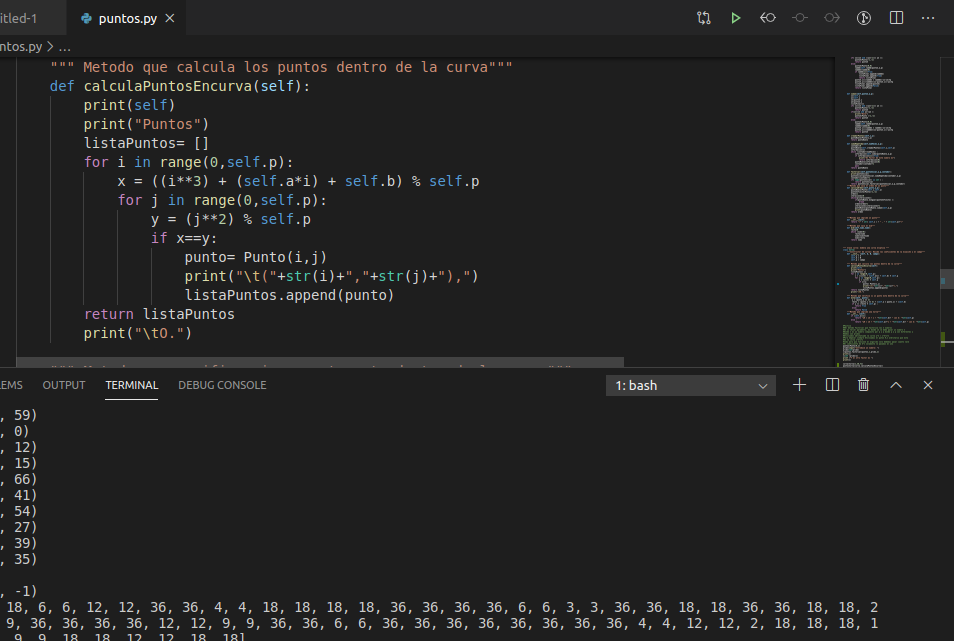
\includegraphics[width=0.7\textwidth]{CalculaPuntos.png}
\caption{CalculaPuntos}
\label{fig:orden}
\end{figure}

\begin{figure}
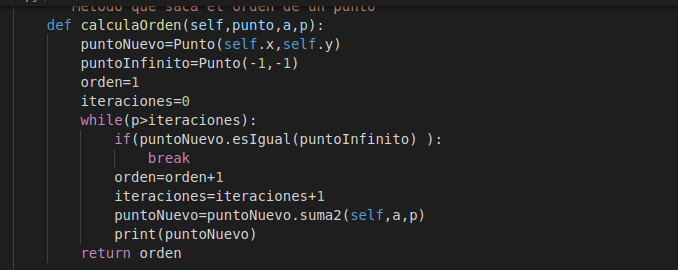
\includegraphics[width=0.7\textwidth]{orden.png}
\caption{orden}
\label{fig:orden}

\end{figure}

Y para realizar la suma de puntos utilizábamos este método que creamos en una clase puntos se puede ver en la imagen de suma.  
\begin{figure}
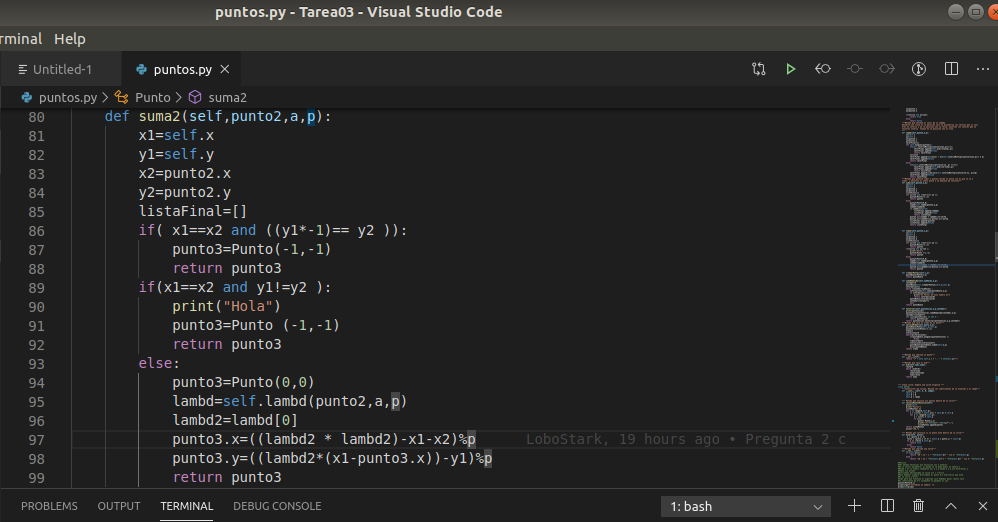
\includegraphics[width=0.7\textwidth]{suma.png}
\caption{suma}
\label{fig:orden}

Ahora usando este codigo podemos decir que un punto que tiene orden 36 es aquel que se encuentra en la sexta posición de la lista es decir el punto (6,45) 
\end{figure}
\end{itemize}
\newpage
\item Sea E :$y^{2}-2=x^{3}+333x$ sobre $\mathbb{F}_{347}$ y sea P = (110,136).
\begin{itemize}
\item[a)] ¿Es Q=(81,-176) un punto de E?\\
\\Para verificar esto hay que sustituir en E Q, \\
(-176$)^{2} - 2= (81)^{3} + 333(81) $\\
30976 - 2 = 531441 + 26973. \\
30974 = 558414 mod 347 \\
Entonces 347$|$558414 - 30974 = 1520, P $\in F_{347}$
\\
\item[b)] si sabemos que $|E| = 358$ ¿Podemos decir E es criptográficamente útil?
¿Cuál es el orden de P? ¿Entre que valores se puede escojer la clave privada?
\\\\El orden de P = 179. E no es criptográficamente útil, ya que no es capaz de dividir a un número primo grande, este número se determina por 172*2, siendo 2 nuestro primo.\\
\item[c)] si tu clave privada es k=101 y algún conocido te ha enviado el mensaje cifrado (M$_1$=(232,278) y M$_2$=(135,214)) ¿Cuál era el mensaje original?\\\\
$M=M_2 - kM_1$\\
$M=(135,214)-101(232,278)$\\
aplicando sumas consecutivas -101(232,278) = (275,176)\\
$M =(135,214)-(275,176)$\\
$M =(135,214)+(275,-176)$\\
$M =(74,87)$ mensaje original\\

\end{itemize}
\item Sea $\mathbb{E}$ : F(x,y)=$y^{2}-x^{3}-2x-7$ sobre $\mathbb{Z}_{31}$ con $\neq \mathbb{E}$ = 39 y P = (2,9) es un punto de orden 39 sobre $\mathbb{E}$, el ECIES simplifado definido sobre $\mathbb{E}$ tiene $\mathbb{Z}^{*}_{31}$ como espacio de texto plano, supongamos que la clave privada es m = 8.
\begin{itemize}
\item[a)] Calcula Q=mP\\
Hay que calcular Q = 8P\\$ ~~~~~~~~~~~~~~~~~~~~~~~~~~~$= 4P + 4P = (2P+2P) + (2P+2P)\\\\
Como son los mismos puntos tenemos $\lambda$ = (3$x_{1}^{2}$ + A) $(2y_{1})^{-1}$ = $(3(2)^{2} + 2)(2(9))^{-1}$ hay que encontrar el inverso de 9 mod 31 usando el algoritmo extendido de euclides, 2(9)$^{-1}$ $\equiv$ 18$^{-1} \equiv $ 19 mod 31.\\
Entonces $\lambda$ = (12+2) x 19 = 266.\\
Queda calcular $x_{3}$ = $\lambda^{2} - x_{1} - x_{2}$, y$_3$ = $\lambda(x_{1} - x_{3}) - y_{1}$.
\\
\\x$_{3}$ = $(266)^{2}$ - 2 - 2 = 70,756-4 = 70,752 $\equiv$ 10 mod 31.
\\y$_{3}$ = 266(2-70752) - 9 = -18,819,509 $\equiv$  2 mod 31.\\
Entonces 2P = (10,2).\\
4P = 2P + 2P =  (10,2)+(10,2).\\
Entonces $\lambda$ = (3(10$^{2}$) + 2)(2(2)$)^{-1}$ = 2,416.\\
x$_{3}$ = (2,416)$^{2}$ -10 -10 = 5,837,036 $\equiv$ 15 mod 31.\\
y$_{3}$ = 2,416(10 - 5,837,036) - 2 = -14102254818 $\equiv$ 8 mod 31.\\
Por lo que 4P = (15,8), solo falta calcular 8P = 4P + 4P = (15,8) + (15,8).\\
Ahora $\lambda$ = (3(15)$^{2}$ + 2)(2(8)$^{-1}$); 2(8)$^{-1} \equiv $ 2 mod 31. \\
entonces $\lambda$ = 677 x 2 = 1354.\\
x$_{3}$ = 1,354$^{2}$ - 15 -15 = 1.833,286 $\equiv$ 8 mod 31.\\
y$_{3}$ = 1354(15 - 1,833,286 )-8 = -24,82,248,942 $\equiv$ 15 mod 31.\\
Entonces 8P = (8,15).
\item[b)] Descifra la siguiente cadena de texto cifrado: \\
((18,1),21),((3,1),18),((17,0),19),((28,0),8)\\
E : y$^{2} = x^{3} + 2x + 7$ mod 31
\begin{itemize}
\item[1)] ((18,1),21)\\
Evaluamos 18 en E:\\
Entonces 18$^{3} +2(18) + 7 = 5875 \equiv $16 mod 31.\\
y = $\pm$ 4, ahora hay que fijarnos en la segunda entrada la cual nos dice que y $\equiv$ 1 mod 2, entonces y = 27.\\
El punto de descompresión es (18,27), entonces 8(18,27) = (15,8)\\
Ahora hay que encontrar 15$^{-1} \equiv $ 29 mod 31,y con esto hay que calcular 29(21) mod 31 que nos da: 20.
\item[2)] ((3,1),18)\\
Evaluamos 3 en E :\\
Entonces 3$^{3} + 2(3) + 7 = 40 \equiv $ 9 mod 31\\
y = $\pm$ 3, ahora hay que fijarnos en la segunda entrada la cual nos dice que y $\equiv$ 1 mod 2, entonces y = 28 \\ 
El punto de descompresión es (3,28), entonces 8(3,28) = (2,22)\\
Ahora hay que encontrar 2$^{-1} \equiv$ 16 mod 31, y con esto hay que calcular 16(18) mod 31 que nos da: 9.
\item[3)] ((17,0),19)\\
Evaluamos 17 en E:\\
Entonces 17$^{3} + 2(17) + 7 = 4954 \equiv$ 25 mod 31\\
y = $\pm$ 5, ahora hay que fijarnos en la segunda entrada la cual nos dice que y $\equiv$ 0 mod 2, entonces y = 26\\
El Punto de descompresión es (17,26) ,entonces 8(17,26) = (30,29)\\
Ahora hay que encontrar 30$^{-1} \equiv$ 30 mod 31, y con esto hay que calcuar 30(19) mod 31 que nos da: 12 %%era 6 y 
\item[4)] ((28,0),8) \\
Evaluamos 28 en E:\\
Entonces 28$^{3} + 2(28) + 7 = 22015 \equiv $5 mod 31
Hay que sumarle a 5, 31 tantas veces como sea necesario para que nos genere un cuadrado perfecto. En este caso 5 + 31 = 36.\\
Entonces y = $\pm$ 6, ahora nos fijamos en la segunda entrada la cual nos dice que y $\equiv$ 0 mod 2, entonces  y = 25\\
El punto de descompresión es (28,26), entonces 8(28,25) = (14,12)\\
Ahora hay que encontrar 14$^{-1} \equiv$ 20 mod 31, y con esto hay que calcular 20(8) mod 31 que nos da: 5.


\end{itemize}
\item[c)] Supongamos que cada texto plano representa un caracter alfabético, convierte el texto plano en una palabra en ingles, usa la asociación (A $\rightarrow$ 1, ... , Z $\rightarrow$ 26) en este caso 0 no es considerado como un texto plano o par ordenado.\\
Del ejercicio anterior obtuvimos los valores $\lbrace 20, 9,12,5 \rbrace$\\
\begin{center}
\begin{tabular}{|c|c|c|c|c|c|c|c|c|c|c|c|c|c|}
\hline
A & B & C & D & E & F & G & H & I & J & K & L & M \\
\hline
1 & 2 & 3 & 4 & 5 & 6 & 7 & 8 & 9 & 10 & 11 & 12 & 13\\
\hline 
N & O & P & Q & R & S & T & U & V & W & X & Y & Z \\
\hline
14 & 15 & 16 & 17 & 18 & 19 & 20 & 21 & 22 & 23 & 24 & 25 & 26\\
\hline 
\end{tabular}
\end{center}
\begin{center}
Y con los valores obtenemos: \textbf{TILE} como mensaje descifrado.
\end{center}
\end{itemize}
\end{enumerate}
\end{document}